% Created 2021-09-27 Mon 12:00
% Intended LaTeX compiler: xelatex
\documentclass[letterpaper]{article}
\usepackage{graphicx}
\usepackage{grffile}
\usepackage{longtable}
\usepackage{wrapfig}
\usepackage{rotating}
\usepackage[normalem]{ulem}
\usepackage{amsmath}
\usepackage{textcomp}
\usepackage{amssymb}
\usepackage{capt-of}
\usepackage{hyperref}
\setlength{\parindent}{0pt}
\usepackage[margin=1in]{geometry}
\usepackage{fontspec}
\usepackage{svg}
\usepackage{cancel}
\usepackage{indentfirst}
\setmainfont[ItalicFont = LiberationSans-Italic, BoldFont = LiberationSans-Bold, BoldItalicFont = LiberationSans-BoldItalic]{LiberationSans}
\newfontfamily\NHLight[ItalicFont = LiberationSansNarrow-Italic, BoldFont       = LiberationSansNarrow-Bold, BoldItalicFont = LiberationSansNarrow-BoldItalic]{LiberationSansNarrow}
\newcommand\textrmlf[1]{{\NHLight#1}}
\newcommand\textitlf[1]{{\NHLight\itshape#1}}
\let\textbflf\textrm
\newcommand\textulf[1]{{\NHLight\bfseries#1}}
\newcommand\textuitlf[1]{{\NHLight\bfseries\itshape#1}}
\usepackage{fancyhdr}
\pagestyle{fancy}
\usepackage{titlesec}
\usepackage{titling}
\makeatletter
\lhead{\textbf{\@title}}
\makeatother
\rhead{\textrmlf{Compiled} \today}
\lfoot{\theauthor\ \textbullet \ \textbf{2021-2022}}
\cfoot{}
\rfoot{\textrmlf{Page} \thepage}
\renewcommand{\tableofcontents}{}
\titleformat{\section} {\Large} {\textrmlf{\thesection} {|}} {0.3em} {\textbf}
\titleformat{\subsection} {\large} {\textrmlf{\thesubsection} {|}} {0.2em} {\textbf}
\titleformat{\subsubsection} {\large} {\textrmlf{\thesubsubsection} {|}} {0.1em} {\textbf}
\setlength{\parskip}{0.45em}
\renewcommand\maketitle{}
\author{Houjun Liu}
\date{\today}
\title{Roberts Ch. 5}
\hypersetup{
 pdfauthor={Houjun Liu},
 pdftitle={Roberts Ch. 5},
 pdfkeywords={},
 pdfsubject={},
 pdfcreator={Emacs 28.0.50 (Org mode 9.4.4)}, 
 pdflang={English}}
\begin{document}

\tableofcontents



\section{Roberts Ch. 5}
\label{sec:orge2c2db0}
\#disorganized

\subsection{India}
\label{sec:org0316c4e}
\begin{itemize}
\item England challenged the "Indian Ocean supremacy"

\begin{itemize}
\item England had before sought to enter spice trade of India, but had
issues trying to do so
\item Had French interference when trying to do business in India
\item For a century held only Fort St. George and Bombay
\item Conducted trade in Coffee and Textiles
\end{itemize}

\item Coffee!

\begin{itemize}
\item Establishment of coffee-houses of London brought popularity of the
drink
\item Tea drinking was also growing at the time
\end{itemize}

\item Company growth

\begin{itemize}
\item East India Co. 1689 defeat pivoted direction to use non-force
strategies
\item Collapse of Mughals after 1707 brought energy and land to the
British Trade

\begin{itemize}
\item Increased polarity between the Marathas Hindus and the Mughals
caused distress
\item Sikhs formed their own sect of Hinduism, detaching from both true
Hindu ideology and Islamic ideology
\item 1730s Persian invasion caused loss in territory
\end{itemize}

\item Britian did not invade the Indian region until much later than the
1740s => CLAIM: because it considered trade very important

\begin{itemize}
\item Finally decided to take action due to CLAIM: hostility towards the
French
\item Ownership of station at Calcutta provided access to riches part of
India
\item Wanted not to interfere with Indian politics, and instead employ
the Mughal model of acceptance-and-profit
\end{itemize}

\item British vs French conflict

\begin{itemize}
\item Supported opposite Indian princes
\item Brought armed struggle between French and British forces
\item French governor Dupleix controlled brilliantly, but was recalled
\item Provincial government of Bengal attacked + captured Calcutta
\item East India Co.'s army recaptured the city + recaptured both
territory of he French and of the governors
\item Recapturing opened the way to British monopoly in India +
diminishing of French dominance
\end{itemize}

\item British Raj

\begin{itemize}
\item Britian proper sent an army to India, legetimizing the corporate
armies of the Co.
\item Taking over Mughal government services @sushu

\begin{itemize}
\item TAX FARMING: government gives a person right to collect taxes
\end{itemize}

\item The Co. formally became ruler of Bengal in 1764

\begin{itemize}
\item French bases became scattered/useless
\item Peace of 1763 left only 5 French trading posts
\item 1769 Compagnie des Indies dissolved
\end{itemize}

\item Took Cerlon from Dutch year after \#verify?
\item Growth => Decline

\begin{itemize}
\item The company turned a bit too territorialist
\item Gave employees too many opportunities to cheat/bribe, and not
enough profit for the company itself
\item British government began nationalizing

\begin{itemize}
\item Set up system of "dual control" in 1784 => lasted until 1858
\end{itemize}
\end{itemize}
\end{itemize}
\end{itemize}

\item Britian successful because of the tax-and-spend cycle

\begin{itemize}
\item Heavy tax to citizen
\item Use tax to fund expansion
\item Citizens get benefit of expansion + don't mind high taxes
\end{itemize}

\item Obviously, this works only if your contry is merchatilist where
\end{itemize}

\begin{figure}[htbp]
\centering
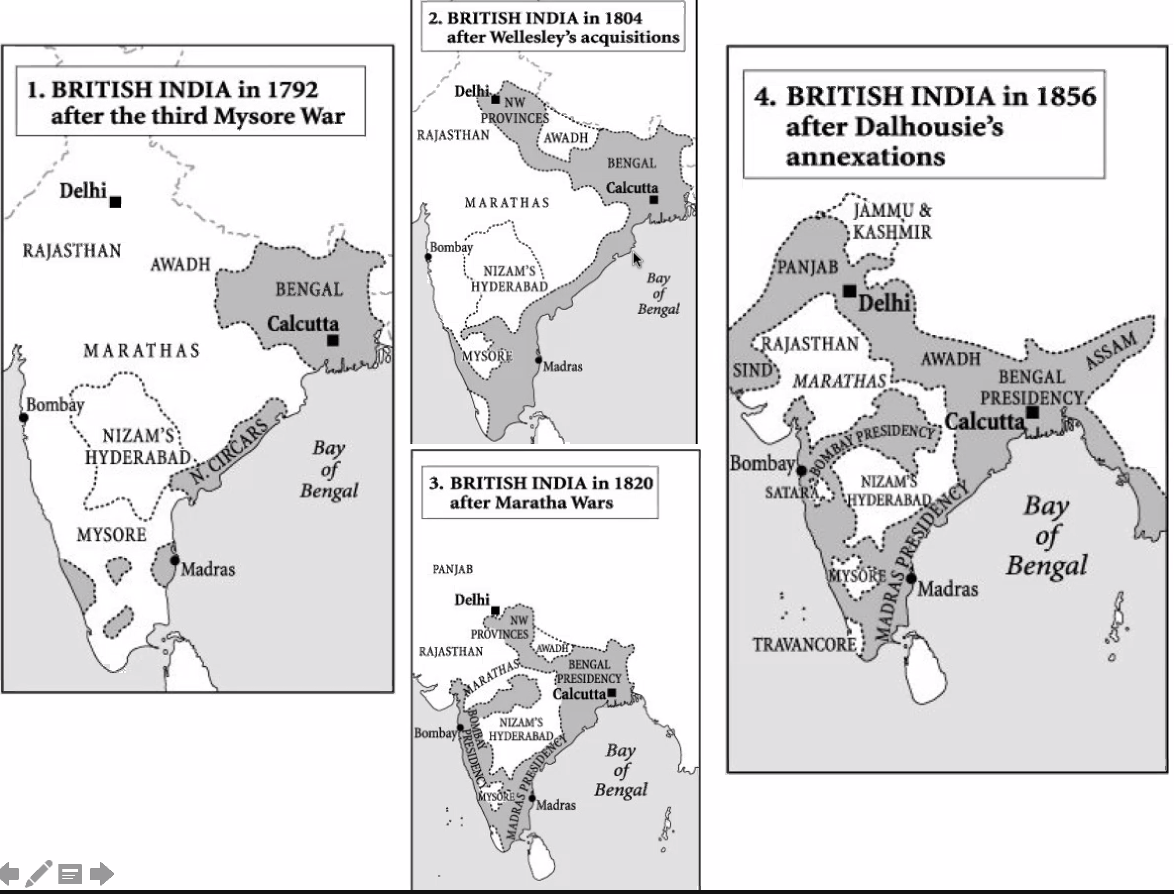
\includegraphics[width=.9\linewidth]{britsacquireinda.png}
\caption{britsacquireinda.png}
\end{figure}

\begin{itemize}
\item Roberts => empirization is because of increased commercial opportunity

\item Trauttmann => empirization is due to the faliture of the silent Dutch
model

\item Salt hedge

\begin{itemize}
\item Salt in + opium out
\item 400 miles (SF:Chicago)
\item Controlled the economy
\end{itemize}
\end{itemize}

\subsection{Carribeans}
\label{sec:org18fec93}
\begin{itemize}
\item Brazil and Carribeans boomed due to sugar crops
\item Main crops: tobacco, hardwood, coffee
\item Spanish influence on Caribbean agriculture

\begin{itemize}
\item Began with growth of fruit + cattle
\item Sugar and Rice was then introduced, but production was slow
\end{itemize}

\item European settlements later appeared with the usual suspects =>
Netherlands, England, French * England established 2 colonies =>
St. Christopher + Barbados * St. Christopher => 3000, Barbados => 2000

\begin{itemize}
\item Early successes due to tobacco: "tobacco colonies"

\begin{itemize}
\item Supplied great customs values to England
\item Left the French with 7,000 and England, 50,000 in the island
\end{itemize}

\item Introduction of sugar crops lead to shift towards Slave trade

\begin{itemize}
\item Tobacco economical if cultivated in small quantities
\item Sugar needed large plantation
\item => Contributed to the overall demographic change in North America
\end{itemize}

\item Spanish control now vested on its control of the slave trade
\end{itemize}

\item Eventually, North Amercia emerged to be a bigger economy than that of
new Spain
\end{itemize}

\subsection{Impacts}
\label{sec:orgbd2472d}
\begin{itemize}
\item Colonies had extracted varied economic benefit from their colonies

\begin{itemize}
\item Spanish => Silver from South America: broke the world economy
\item England => Stimulated European exports + manufacturing: leading
people to flow from Europe to Africa to Asia
\item CLAIM: colonization of Americas brought huge, incalculable economic
benefits
\end{itemize}

\item The Western hemisphere is decidedly European

\begin{itemize}
\item Organized under European legal system
\item Christanized
\end{itemize}
\end{itemize}

\begin{quote}
Europeans did not just conquer; they exterminated local cultures and
peoples and replaced them with their own.
\end{quote}

\begin{itemize}
\item The older Amercian cultures cut off from populating other parts of the
world
\item CLAIM: the European dominance was a sign to "Asian Nationalists"
(Japan??) as the sign of European injustice
\item Americas suffered some species going extinct, and yet others massively
planted

\begin{itemize}
\item Plants

\begin{itemize}
\item Potato
\item Sweet potato
\item Maize
\end{itemize}

\item Domesticated Animals

\begin{itemize}
\item Pigs
\item Sheep
\item Chicken
\end{itemize}

\item => "Colombian exchange"
\end{itemize}
\end{itemize}
\end{document}
